\section{Proposed Methodology}
\label{sec:pipeline}
 \textit{Defects4J v2.0} \cite{just2014defects4j} dataset provides over 830 reproducible bugs curated across 17 real world Java projects. In this research, we classify every \textit{Defects4J} bug into an ODC defect type using an LLM following three stages including Data Collection, Bug Classification, and Evaluation. The primary goal of this research is to identify and categorize software defects based on their underlying characteristics, thereby providing a structured understanding of the nature and distribution of defects in \textit{Defects4J} dataset. The data collection stage prepares and transforms the \textit{Defects4J} bug data into a suitable representation for classification; the classification stage assigns appropriate ODC types to the identified bugs; and the evaluation stage assesses the performance and reliability of the classification results using appropriate evaluation measures. Figure~\ref{fig:architecture} demonstrates the workflow in detail, and the rest of this section walks through each of the three stages in turn. 

\textcolor{red}{move the following part in other sections of the methodology, where appropriate. commented out for now}
%First, in \emph{preprocessing}, we build the bug a case file: the report, the failing tests, the error messages, and the code around them, exactly what a developer would look at before reading the fix. Second, in \emph{classification}, we hand that case file to a large language model and ask it to assign an ODC defect type, using one of three prompting strategies that range from a single quick guess to an enforced, evidence-driven reasoning loop. Third, in \emph{evaluation}, because \textit{Defects4J} carries no official ODC answer key, we check the classification against itself: we classify the same bug a second time after showing the model the real fix, and measure how closely the early, symptom-only classification matches the later, fix-informed one.

\begin{figure*}[t]
    \centering
    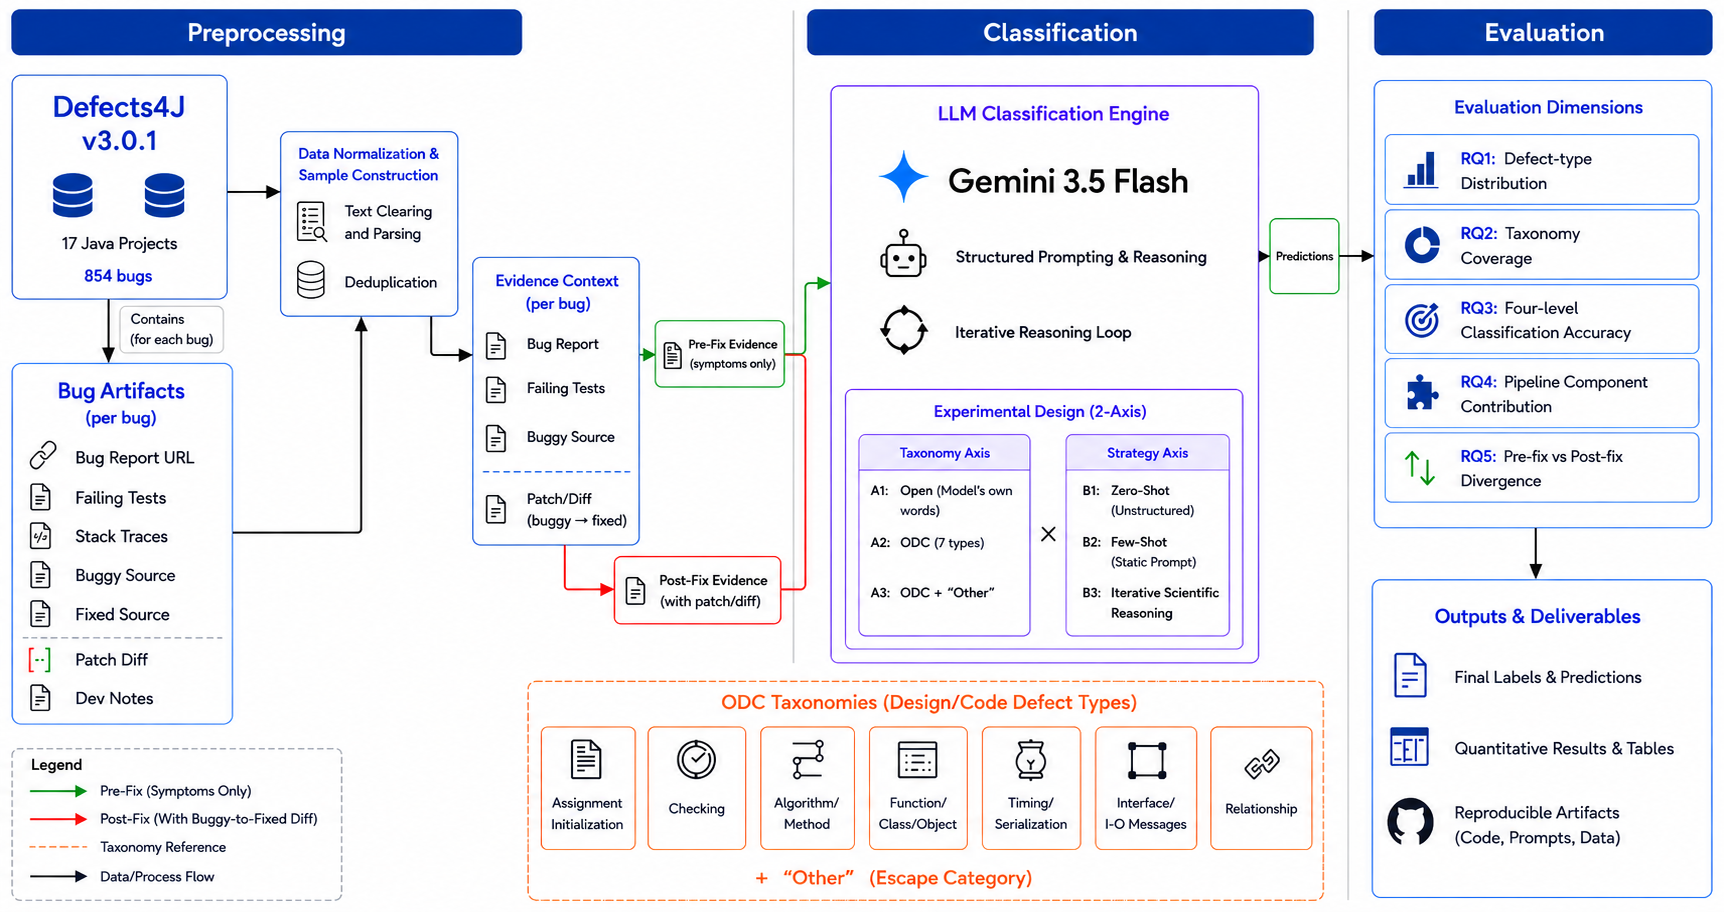
\includegraphics[width=\textwidth]{sections/methodologyFIG.png}
    \caption{Overview of the proposed methodology for preprocessing, ODC classification, and evaluation.}
    \label{fig:methodology}
\end{figure*}


\subsection{Data Collection}
\label{subsec:collection}
To classify \textit{Defects4J} bug to ODC type using LLM we prepared two types of files namely - pre-fix context and post-fix context for the buggy and fixed version of the code receptively. The only difference between these two files is fix diff which represents the exact difference between a buggy version of code and its fixed version. These two files will be fed to an LLM to provide necessary context to classify the bug automatically. \textcolor{red}{normalization, deduplication}

Bug classification should be performed solely using the pre-fix context, without access to any information from the corresponding fix. Since the \textit{Defects4J} dataset does not include ground-truth ODC defect type labels, we evaluate our approach by using the post-fix context, where the actual code changes provide sufficient evidence for defect type classification.

For each bug we extract and store the following artifacts as a context for LLM to classify \textit{Defects4J} bug to ODC bug type.  

\paragraph{Bug identity and Defects4J metadata}
We record the project and bug IDs, the buggy and the
fixed-version revision from Defects4J, the issue-tracker report ID and URL,
the ground-truth modified class(es), and the triggering and relevant tests.

\paragraph{Bug report Content}
We fetch the original bug report from the issue tracker and store it in
full, including its title, labels, and comment thread.

% \paragraph{Checkout, build, and reproduction}
% We check out the buggy revision, record the directory layout and classpaths,
% then compile and run the test suite, logging exit codes to confirm the bug
% still reproduces.

\paragraph{Failing tests, exception, and stack trace}
For each triggering test, we capture its name, the raised exception, the raw
stack trace, and a parsed list of every frame (class, method, file, line).

\textcolor{red}{Highlight this part: What is Suspicious frames, how extracted, why used?}
\paragraph{Suspicious frames}
We keep only the frames pointing into the project's own source, discarding
JUnit, Ant, and JDK frames; these anchor the snippet-extraction step.

\paragraph{Code snippets}
Around each suspicious frame and each failing test, we cut a short source
window with the offending line marked, giving localized context.

\paragraph{Hidden oracles}
We separately store the ground-truth modified class(es) as a hidden oracle,
excluded from the LLM-facing prompt and used only later for evaluation.

\paragraph{Fix diff (post-fix oracle)}
For post-fix evaluation we also record the buggy-to-fixed source diff, left
empty in the pre-fix record and withheld from the model otherwise.

%\paragraph{Keeping the fix out of the pre-fix evidence.}
%A pre-fix classification is only meaningful if it genuinely cannot see the fix. Two things can leak fix knowledge by accident: the raw \textit{Defects4J} metadata names the classes the fix touched, and bug-report text for already-resolved issues often discusses the resolution. We strip both from the pre-fix evidence right before it is shown to the model, while leaving the post-fix evidence untouched, since that arm is allowed to know the fix. This gives us two versions of the same case file that differ in exactly one respect, the fix diff, which is precisely what the pre-fix/post-fix comparison in Section~\ref{sec:eval} is designed to isolate.

\paragraph{ODC Attribute to Defects4J Artifact  Mapping.}
Among the eight attributes (Subsection \ref{subsec:ODC}) of ODC, we considered only \textit{Defect Type} and \textit{Impact}, as these are the only attributes that can be reliably inferred from the evidence available in the Defects4J dataset. 
%Each maps onto a specific part of what \textit{Defects4J} gives us for a bug. The failing tests, their exception and stack trace, and the surrounding source feed \textbf{Defect Type}; the bug report and the observed failure feed \textbf{Impact}.

\textcolor{blue}{
\textbf{Defect Type} is the study's main target, and we extract it under both
settings: the pre-fix setting, using symptom-only evidence, which is the central
task, and the post-fix setting, using that same evidence plus the real fix diff,
given as oracle information. Neither setting reads a label mechanically off the
patch; the post-fix setting serves only as an upper reference point, not as
ground truth.}

\textcolor{red}{Defect Type is classified using the technical evidence generated during bug reproduction, including the failing test cases, exception information, stack trace, and the relevant source code context surrounding the failure. These artifacts provide insight into the underlying cause of the defect, making them suitable for identifying its defect type.}

\textcolor{blue}{
\textbf{Impact} is the only attribute we claim to detect at discovery time. We
give the model all thirteen \textbf{ODC impact categories} plus an \texttt{Unknown} option
and ask it to pick exactly one, based only on the bug report and the observed
failure, never on how the bug was actually fixed. The response schema accepts no
other label, no free-text reaches our analysis. The \textit{zero-free}
strategy (Section~\ref{sec:strategies}) is the exception: it must avoid ODC terms
by design, so we withhold this vocabulary from it.}

\textcolor{red}{is determined from the bug report and the observed failure, as these describe the externally visible effect of the defect on the system rather than its implementation details.}

\subsection{LLM-based ODC Classification}
\label{subsec:classification}
In the classification stage \textit{Defect4J} bugs are classified into ODC types using Gemini 3.5 Flash model. The model was fed two type of contexts (pre-fix and Post-fix) collected during the data collection stage. The contexts are provided to the model using three types of promoting strategy - zero shot, few shot and ............... . 

\paragraph{Prompting Strategy} We fed two types of contexts collected in the data collection stage into an LLM. Two types of prompts have been created for this classification - system prompt and user prompt. \textcolor{red}{System prompt is used for .......... User prompt is used for ...........} These two types of prompts were employed in three prompting startegies - Zero Shot, few shot and .......

%With the case file ready, the model has to produce a classification. We tried three different ways of asking it to reason, and for each way, we also tried different ways of constraining its vocabulary. Not every combination is sensible: a single quick guess cannot be paired with a fixed list of types it is never shown, so in practice we only use five combinations in this study, and the one we rely on by default pairs the most open vocabulary with the most demanding reasoning strategy. We lay out the full space of combinations, and why we chose that default, in Section~\ref{sec:results} alongside the results it produces.

\paragraph{How strict the vocabulary is.}
The model can answer in three ways. Under the \textit{closed} setting, it must
pick exactly one of the seven canonical ODC Design/Code types. Under the
\textit{open} setting, it may instead say ``Other'', but only together with a
written justification, its best guess at the nearest of the seven types, and a
confidence score, so every escape is auditable rather than a shrug. Under the
\textit{free} setting, it answers in its own words with no fixed list at all,
which lets us later measure how much a taxonomy narrows down an otherwise
sprawling vocabulary. Whenever a fixed list is in play, the model also returns a
small structured record alongside its answer: the chosen type, any close
alternatives, the broader ODC family the type belongs to, a confidence score, and
a short trace of its reasoning.

\paragraph{Zero: a single quick guess.}
The simplest strategy is one plain prompt with no taxonomy and no examples. It is
the unstructured baseline every other strategy is measured against.

\paragraph{Few: one strong, well-prepared prompt.}
The second strategy still asks for only one answer, but we build the prompt
carefully: it defines every ODC type with example patterns, warns the model away
from defaulting to the vague, catch-all Function/Class/Object type, walks
through a short decision checklist before that catch-all type is even allowed
to be considered, and includes a handful of worked examples we chose
specifically for pairs of types that are easy to confuse. This is the strongest
single-shot prompt we could build, and it is the fair baseline the third
strategy has to beat.

\paragraph{Scientific: an enforced reasoning loop.}
The third strategy does not let the model simply narrate a chain of thought and
call it done. We borrow the loop structure of scientific debugging and adapt it
from finding a fault to naming its type: on every turn, the model must propose a
hypothesis about the defect type; predict what specific evidence would have to
be true if that hypothesis were correct; ask for exactly that piece of evidence
from the case file, evidence it has not yet been shown; read what comes back and
judge whether it supports or contradicts the hypothesis; and either conclude,
once the evidence is sufficient, or start another turn, up to six in total.
Figure~\ref{fig:architecture} shows this loop as part of the full
pipeline; the zero and few strategies above are, by comparison, a single step
each. Because the model has to commit to a prediction before it is allowed to
see the evidence that would confirm or deny it, this strategy cannot simply
rationalise a first guess after the fact, which is exactly what distinguishes
it from the other two.

\begin{figure}[H]
\centering
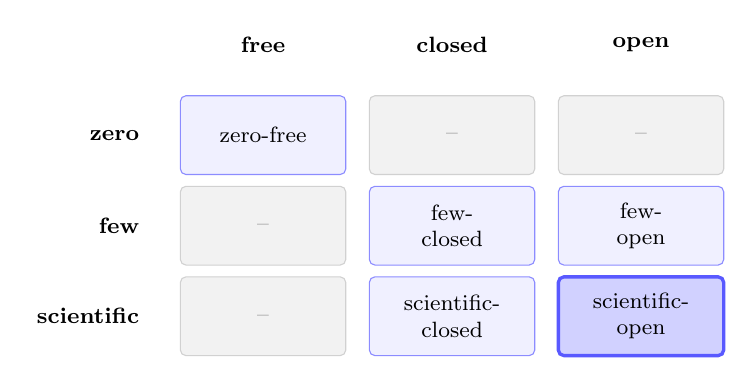
\begin{tikzpicture}[
  font=\footnotesize,
  cell/.style={rectangle, rounded corners=2pt, minimum width=2.1cm,
               minimum height=1.0cm, align=center, draw},
  valid/.style={cell, fill=blue!6,  draw=blue!45},
  def/.style={cell,   fill=blue!18, draw=blue!65, very thick},
  invalid/.style={cell, fill=black!5, draw=black!18, text=black!45},
  hdr/.style={align=center, font=\footnotesize\bfseries}
]
% column headers (taxonomy)
\node[hdr] at (0,1.15)   {free};
\node[hdr] at (2.4,1.15) {closed};
\node[hdr] at (4.8,1.15) {open};
% row headers (strategy)
\node[hdr, anchor=east] at (-1.45, 0)    {zero};
\node[hdr, anchor=east] at (-1.45,-1.15) {few};
\node[hdr, anchor=east] at (-1.45,-2.30) {scientific};
% grid
\node[valid]   at (0,0)      {zero-free};
\node[invalid] at (2.4,0)    {--};
\node[invalid] at (4.8,0)    {--};
\node[invalid] at (0,-1.15)  {--};
\node[valid]   at (2.4,-1.15){few-\\closed};
\node[valid]   at (4.8,-1.15){few-\\open};
\node[invalid] at (0,-2.30)  {--};
\node[valid]   at (2.4,-2.30){scientific-\\closed};
\node[def]     at (4.8,-2.30){scientific-\\open};
\end{tikzpicture}
\caption{The three classification strategies (rows) crossed with the three
         vocabulary settings (columns). Five of the nine cells are valid; the
         four grey cells are invalid combinations, since \textit{zero} carries
         no vocabulary constraint and \textit{free} defines none.
         \textit{scientific-open} (bold) is the default for both pre-fix and
         post-fix evidence.}
\label{fig:conditions}
\end{figure}

\paragraph{Cleaning up the answer.}
Whatever the model returns is checked before it is trusted: we confirm the type
is one of the seven canonical names, or a properly justified ``Other''; clamp the
confidence score into a sensible range; recompute the broader family from the
chosen type ourselves rather than trusting the model's own labelling; and tidy up
the alternative-type and reasoning fields so every artefact downstream has the
same shape. This keeps a malformed or inconsistent answer from quietly
corrupting the results.

\subsection{Evaluation}
\label{sec:eval}

The last step asks a simple question: how much do we trust the classification?
\textit{Defects4J} gives us no official ODC answer key, so instead of measuring
against ground truth, we measure a classification against itself under better
information. We take the pre-fix classification, symptoms only, and compare it
with the post-fix classification of the same bug, which additionally saw the
real fix. We compare the two at four levels of strictness, from the strictest
to the most
forgiving: exact agreement on the primary type; agreement once each side's list
of close alternatives is allowed; agreement at the level of the broader ODC
family rather than the exact type; and Cohen's~$\kappa$,
\begin{equation}
  \kappa = \frac{p_o - p_e}{1 - p_e},
  \label{eq:kappa}
\end{equation}
a chance-corrected agreement score computed from the observed agreement $p_o$ and
the agreement $p_e$ expected by chance alone, read on the standard scale where
$\kappa \ge 0.61$ counts as substantial agreement \citep{landis1977measurement}.
A tiered comparison matters here because even trained human ODC experts disagree
on a meaningful share of real cases, so a single strict-match number would
understate how reasonable the model's classifications actually are.

The remaining RQs reuse this machinery differently: RQ1, RQ3, and RQ5
draw on the same pre-fix/post-fix comparison; RQ2 compares the closed and open
taxonomy passes to see how often the model needs the escape category; and RQ4
compares the three strategies against each other to see how much each narrows
the vocabulary and improves consistency.

